\section{Word Clouds Revisited}
\label{wordcloudsrevisited}
\href{https://open.kattis.com/problems/wordclouds}{View on Kattis}\\
\textbf{Tags:} Dynamic Programming\\
\subsection{Problem Description}
We are given a list of text boxes, represented with a width and a height. We
need to lay them out within a box of fixed width. An entry can either be placed
horizontally to the right of the previous box (if it fits), or at the far left
end of the next row. The height of each row is the sum of the heights of every
entry in the row. Our goal is to minimize the total height of the word cloud.\\

As it turns out, a greedy solution, as shown in Figure
\ref{wordcloudsrevisited:greedy} may not be the optimal solution, depicted in
Figure \ref{wordcloudsrevisited:optimal}

\begin{figure}[h!]
  \centering
  \begin{minipage}{0.45\textwidth}
    \centering
    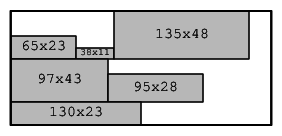
\includegraphics[width=0.9\textwidth]{Images/wordcloudsrevisited-greedy.png}
    \caption{Greedy Strategy}
    \label{wordcloudsrevisited:greedy}
  \end{minipage}
  \hfill
  \begin{minipage}{0.45\textwidth}
    \centering
    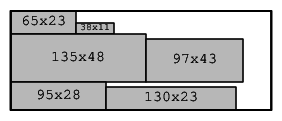
\includegraphics[width=0.9\textwidth]{Images/wordcloudsrevisited-optimal.png}
    \caption{Optimal Solution}
    \label{wordcloudsrevisited:optimal}
  \end{minipage}
\end{figure}

\subsection{Algorithm}

We can make this problem more tractable using dynamic programming. To approach
this problem with that strategy, we need to define two things: an optimal
substructure, and a data structure for memoizing the result.\\

\textbf{Optimal Substructure}\\
An optimal substructure simply represents some way of breaking the problem into
smaller pieces, or some relation that we can use to build upon previous
solutions to smaller portions of the problem. In this case, we can realize that
we only need to track the smallest total height attainable for every possible
width $j$ of the final column after inserting the $ith$ entry. Then, to
calculate the $i+1$th entry's optimal values, we can iterate over all optimal
solutions to the $i$th case and track the results of both inserting in that row
(if possible) or inserting a new row.\\

\pagebreak

\textbf{Data Structure}\\
If we are given $N$ entries and a width of $W$, one option is to store everything
in an $N \cdot (W+1)$ array. To compute the results of the $i$th row, we can
iterate over all columns of the previous row. However, because many columns in
the previous row may not be attainable, we can instead use a map of integers to
optimal values, allowing us to cut down on the average case complexity.
Additionally, because we only need the $i$th row to calculate the $i + 1$th row,
we only need to keep 2 maps, rather than $N$ of them.\\
\hfill\break
Armed with this, we can arrive at the following psuedocode:
\hfill\break
\begin{algorithmic}
  \State Let $best$ be a map of width to the optimal solution for that width.
  \For{Rectangle $r$ in the input}
    \State Let $nextBest$ be a new map of width to the optimal solution.
    \For{$width$, $solution$ in $best$}
      \State $nextBest(r.width) \gets optimal(nextBest(r.width),
        addNewLine(best(width), r))$
      \If{$r.width + width \leq W$}
        \State $newWidth \gets r.width + width$
        \State $nextBest(newWidth) \gets optimal(nextBest(newWidth),
          addSameLine(best(width), r))$
      \EndIf
    \EndFor
    \State $best \gets nextBest$
  \EndFor
  \State Return smallest height in $best$.
\end{algorithmic}
\hfill\break
The optimal solution is whichever minimizes the total height, while $addNewLine$
and $addSameLine$ can be implemented by following the rules of the layout.\\
\hfill\break
\textbf{Time Complexity:} $\mathcal{O}(N \cdot W)$\\
\textbf{Space Complexity:} $\mathcal{O}(W)$\\
Where $N$ is the number of entries $(2 \leq N \leq 5000)$ and $W$ is the width
of the word cloud $(150 \leq W \leq 1000)$.
\pagebreak
\subsection{Implementation}
\lstinputlisting[
  lastline=45,
  language=Java
]{Solutions/WordCloudsRevisited.java}
\pagebreak
\lstinputlisting[
  firstline=47,
  language=Java
]{Solutions/WordCloudsRevisited.java}
\pagebreak
